\chapter{Проектирование информационной системы «Мессенджер»}

Информационная система «Мессенджер» построена на основе микросервисной архитектуры. Для реализации и серверной и клиентской части информационной системы был выбран язык программирования TypeScript, что позволяет переиспользовать написанный программный код, выделяя некоторые его части в NPM пакеты.

На текущий момент, серверная часть состоит из следующих микросервисов: файловое хранилище, почтовый сервер, сервис с основной бизнес-логикой.

\section{Организация процесса разработки информационной системы}

Для улучшения опыта разработки, в проект заложены основные современные DevOps практики, ускоряющие процесс разработки информационной системы.

DevOps (development \& operations) — методология автоматизации технических процессов сборки, настройки и развертывания программного обеспечения \cite{DevOps}.

В качестве стратегии разработки программного обеспечения была выбрана стратегия монорепозитория. Все сервисы, входящие в информационной систему, разбиты на пакеты и содержаться в одном Git репозитории.

Для управления зависимостями, сборкой, публикацией пакетов, был выбран инструмент Lerna.

Для автоматизации развертывания сервисов используется инструмент Docker, который позволяет «упаковать» сервис вместе со всем его окружением и зависимостями в контейнер, который может быть развернут на любой системы Linux с поддержкой контрольных групп в ядре \cite{Docker}.

Внутри Docker Compose конфигурации объявляются все сервисы информационной системы вместе с их окружением (листинг \ref{ls:docker-compose}).

\begin{lstlisting}[caption={Конфигурация Docker Compose}, label={ls:docker-compose}]
services:
  mongodb:
    image: bitnami/mongodb:latest
    container_name: messenger-mongodb-production
    restart: always
    networks:
      - messenger-network
    volumes:
      - messenger-mongodb:/data/db
    environment:
      MONGODB_DATABASE: messenger
    env_file:
      - packages/backend/configs/.env.production

  backend:
    build:
      context: packages/backend
      dockerfile: Dockerfile
    environment:
      NODE_ENV: production
    container_name: messenger-backend-production
    restart: always
    networks:
      - default
      - messenger-network
    ports:
      - "3000"
      - "8080"
    depends_on:
      - mongodb
  web-app:
    build:
      context: packages/web-app
      dockerfile: Dockerfile
    container_name: messenger-web-app-production
    networks:
      - default
    ports:
      - "80"
    volumes:
      - /data/nginx:/etc/nginx/sites-enabled
    command: nginx -g "daemon off;"
    depends_on:
      - backend
\end{lstlisting}

Для автоматизации непрерывной интеграции и непрерывного развертывания, используется инструмент Gitlab CI. С помощью него реализуется сборка проекта, модульной и интеграционное тестирование, статический анализ кодовой базы, развертывание информационной системы.

CI задания выполняются при каждом изменении кодовой базы, в любых Git ветках. Развертывание выполняется только при изменениях в ветке «main». Всего определено 5 стадий — установка зависимостей, сборка, статический анализ кода, тестирование, развертывание (листинг \ref{ls:gitlab-ci}). Внутрь конфигурации импортируются другие конфигурации Gitlab CI, так, например 	«.write-production-variables» выполняет встраивание из специального хранилища секретных ключей для базы данных, JWT и других инструментов внутрь переменных окружения сервера.

\begin{lstlisting}[caption={Конфигурация Gitlab CI}, label={ls:gitlab-ci}]
stages:
  - setup
  - build
  - linting
  - tests
  - deploy-production

include:
  - '.cache-ci.yml'
  - '.variables-ci.yml'

build-backend:
  stage: build
  script:
    - npx lerna run build --scope=backend
  only:
    changes:
      - packages\backend\**\*

build-web-app:
  stage: build
  script:
    - npx lerna run build --scope=web-app
  only:
    changes:
      - packages\web-app\**\*

linting:
  stage: linting
  script:
    - npx lerna run lint --scope=backend
  only:
    changes:
      - packages\backend\**\*

unit-tests:
  stage: tests
  script:
    - npx lerna run test --scope=backend
  only:
    changes:
      - packages\backend\**\*

deploy-production:
  stage: deploy-production
  extends: .write-production-variables
  image:
    name: docker/compose:latest
  script:
    - docker-compose -f docker-compose.production.yml up --build -d
  only:
    - main
\end{lstlisting}

\section{Проектирование архитектуры серверной части информационной системы}

\subsection{Использоваине метафреймворка Nest.js для создания масштабируемого серверного приложения на платформе Node.js}

В ходе анализа различных Node.js фреймворков, был выбран фреймворк Nest.js, который, на текущий момент, является единственным фреймворков с открытым исходным кодом, предоставляющим готовую архитектуру и инструменты для тестирования, работой с базой данных, валидации входных данных, API-интерфейсы для WebSocket, API-интерфейсы для создания микросервисов.

Nest.js является платформой агностиком, которая может использовать внутри себя веб-сервер Express или Fastify. По сравнению с другими Node.js фреймворками, Nest обеспечивает слой абстракции, что дает возможность легко масштабировать кодовую базу. Условное разделение кодовой базы на слои показано на рисунке \ref{fig:nestjs}. Фреймворк полностью написан на языке TypeScript и сочетает в себе элементы объектно-ориентированного программирования, функционального программирования и функционально-реактивного программирования \cite{Nestjs}.

\begin{figure}[H]
\begin{center}
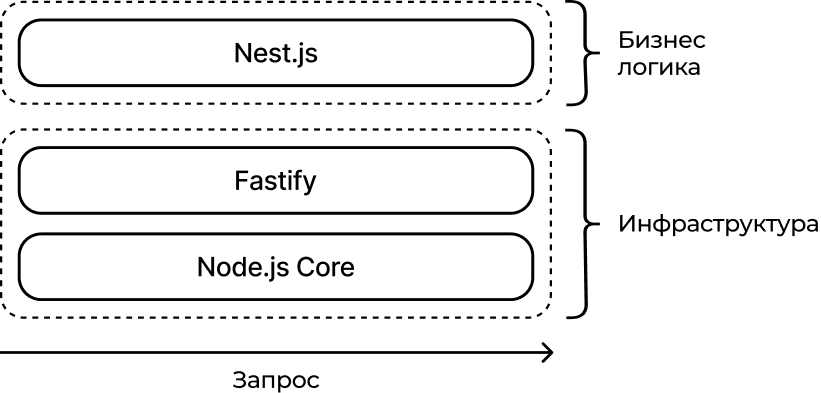
\includegraphics[width=1.0\hsize]{fig/nestjs.png}\\[2mm]
\caption{Разделение кодовой базы веб-сервера на слои}\label{fig:nestjs}
\end{center}
\end{figure}

Вся кодовая база разделяется на модули, которые являются самыми крупными сущностями в разрабатываемом приложении. Позже, некоторые модули могут быть выделены в отдельные микросервисы, для более гибкой балансировки нагрузки на них. В свою очередь внутри модулей могут быть выделены следующие сущности:

\begin{enumerate} 
  \item Контроллеры (Controllers) — отвечает за обработку входящих HTTP запросов.
  
  \item Провайдеры (Providers) — сущности, реализующие определенную бизнес-логику. Ими могут быть сервисы, фабрики, помощники и т.д.

  \item ПО промежуточного слоя (Middleware) — функции, вызывающиеся перед обработчиком маршрута, имеют доступ к объектам запроса и ответа.

  \item Фильтры исключений (Exception filters) — сущности, отвечающие за обработку всех необработанных исключений в приложении.

  \item Трубы (Pipes) — могут иметь два различных варианта использования. Преобразовывать входные данные в желаемую форму. Проверять входные данных и, если они действительны, просто передать их без изменений, в противном случае сгенерировать исключение.

  \item Охранники (Guards) — определяют, будет ли данный запрос обрабатываться обработчиком маршрута или нет, в зависимости от определенных условий, присутствующих во время выполнения.

  \item Перехватчики (Interceptors) — вдохновлены техникой аспектно-ориентированного программирования. Позволяют привязать дополнительную логику до/после выполнения метода, преобразовать результат, возвращаемый функцией, преобразовать исключение, выброшенное из функции, расширить базовое поведение функции, полностью переопределить функцию в зависимости от конкретных условий (например, для целей кэширования).
\end{enumerate}

Все Injectable-сущности (например сервисы, трубы, охранники, и т.д.) можно внедрить как зависимость. Это означает, что объекты могут создавать различные отношения друг с другом, а функция «подключения» экземпляров объектов может быть в значительной степени делегирована системе выполнения Nest.

Nest.js используется концепцию внедрения зависимостей. Внедрение зависимостей — это метод инверсии управления (IoC), при котором создание экземпляров делегируется контейнеру зависимостей IoC вместо того, чтобы выполнять создания зависимостей императивно. Пример того, как внедряются зависимости в Nest.js показан на рисунке \ref{fig:nestjs-ioc}.

\begin{figure}[H]
\begin{center}
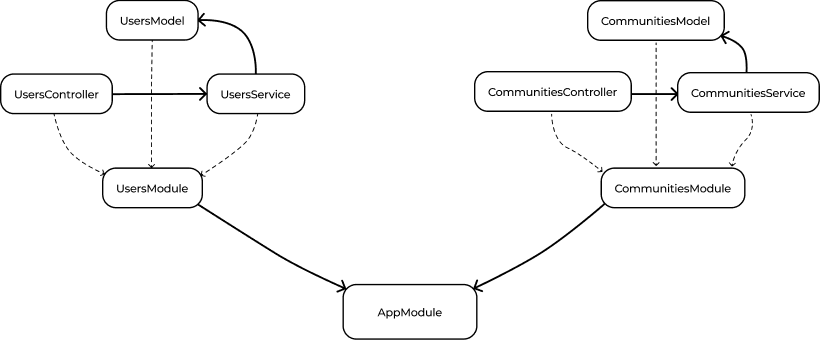
\includegraphics[width=1.0\hsize]{fig/nestjs-ioc.png}\\[2mm]
\caption{Внедрение зависимотей в Nest.js}\label{fig:nestjs-ioc}
\end{center}
\end{figure}

\subsection{Использование системы управления базой данных MongoDB}

MongoDB — кроссплатформенная, документно-ориентированная, NoSQL база данных, предоставляющая возможности индексации и выполнения запросов. Использует JSON схему базы данных. Система масштабируется горизонтально, используя сегментирование объектов баз данных. MongoDB не использует табличное устройство c четко определенным количеством столбцов и типов данных, в отличие от реляционных баз данных. Центральным понятием в документно-ориентированной системе является документ, который можно представить как объект, хранящий некоторую информацию \cite{Mongo}. Структура коллекции MongoDB показана на рисунке \ref{fig:mongodb}.

\begin{figure}[H]
\begin{center}

\includegraphics[width=1.0\hsize]{fig/mongodb.png}\\[2mm]
\caption{Структура коллекции MongoDB}\label{fig:mongodb}
\end{center}
\end{figure}

MongoDB была выбрана в качестве основной СУБД, за счет простого горизонтального масштабирования, предусмотренного разработчиком базы данных и скоростью разработки за счет возможность вложено хранить большие массивы данных. К минусам использования MongoDB можно отнести сложность миграции данных при изменении схем коллекций.

Поскольку MongoDB является СУБД, не требующей строгого определения структуры коллекций, для моделирования данных приложения на основе схемы используется ORM Mongoose. Он включает в себя встроенное приведение типов, валидацию коллекций на основе схем, построение запросов.

Mongoose легко интегрируется в Nest.js как провайдер. Подключение к базе данных выполняется на уровне корневого модуля \verb|AppModule| (листинг \ref{ls:mongoose-module}), схемы могут хранится где угодно и подключаться внутрь модулей, где они вызываются.

\begin{lstlisting}[caption={Подключение MongooseModule в приложение Nest.js}, label={ls:mongoose-module}]
import { Module } from '@nestjs/common';
import { MongooseModule } from '@nestjs/mongoose';

@Module({
  imports: [MongooseModule.forRoot('mongodb://localhost/nest')],
})
export class AppModule {}
\end{lstlisting}

Каждая схема сопоставляется с коллекцией MongoDB и определяет форму документов в этой коллекции. Модели отвечают за создание и чтение документов из MongoDB. Схемы можно создавать с помощью декораторов или императивно с помощью самого Mongoose. Использование декораторов для создания схем значительно сокращает количество шаблонов и улучшает общую читаемость кода (листинг \ref{ls:mongoose-schema}).

\begin{lstlisting}[caption={Создание схемы Mongoose}, label={ls:mongoose-schema}]
import { Prop, Schema, SchemaFactory } from '@nestjs/mongoose';
import { HydratedDocument } from 'mongoose';

export type CatDocument = HydratedDocument<Cat>;

@Schema()
export class Cat {
  @Prop()
  name: string;

  @Prop()
  age: number;

  @Prop()
  breed: string;
}

export const CatSchema = SchemaFactory.createForClass(Cat);
\end{lstlisting}

\subsection{Архитектура сетевого взаимодействия с клиентом на основе протокола WebSocket}

Согласно спецификации, сообщение в протоколе WebSocket представляет собой неопределенные данные любой структуры, поступающие на обработчик сервера \verb|onmessage| (листинг \ref{ls:ws-server-create}).

\begin{lstlisting}[caption={Создание веб-сокет сервера}, label={ls:ws-server-create}]
import { WebSocketServer } from 'ws';

const wss = new WebSocketServer({ port: 8080 });

wss.on('connection', function connection(ws) {
  ws.on('message', function message(data) {
    console.log('received: %s', data);
  });
});
\end{lstlisting}

Для того, чтобы поступающие данных отправлялись на нужные обработчики в подключенных модулях, необходимо определить протокол взаимодействия между веб-сервером и веб-приложением «WSMessenger». Каждое сообщение должно являться объектом, содержащим в себе поле «event», определяющим, на какой обработчик должно быть доставлено сообщение, поле «id», содержащим уникальный идентификатор сообщения, поле «data», содержащим передаваемые данные (листинг \ref{ls:ws-request}).

\begin{lstlisting}[caption={Структура WebSocket запроса}, label={ls:ws-request}]
export interface WsRequest<T = unknown> {
  event: string;
  id: string;
  data: T;
}
\end{lstlisting}

По умолчанию, по соединению WebSocket передаются текстовые данные, обычно в формате JSON, которые сериализуются в объекты при получении сообщения. В разрабатываемом протоколе, данные будут передаваться в двоичной форме с типом ArrayBuffer для того, чтобы увеличить скорость передачи данных за счет сжатия и скорости сериализации и десериализации.

В Nest.js существуют определенная сущность, обрабатывающая WebSocket сообщения — «Gateway» (шлюз). Nest.js абстрагируется от деталей реализации, поэтому все основные концепции и сущности рассмотренные ранее, работают со шлюзом также, как с обычным HTTP контроллером.

Передача данных в шлюзы обеспечивается WebSocket адаптером, который находится на инфраструктурном уровне, он представляет собой WebSocket сервер, запускающийся во время старта приложения.

Для веб-сервера информационной системы «Мессенджер» был разработан собственный WebSocket адаптер на основе Node.js библиотеки «ws», определяющей WebSocket сервер. Разработанный адаптер принимает и отправляет сообщения в бинарном виде, а также использует алгоритм сжатия сообщений (листинг \ref{ls:ws-adapter}).

\begin{lstlisting}[caption={Метод WebSocket адаптера передающий поступающие сообщения на шлюзы Nest.js}, label={ls:ws-adapter}]
public bindMessageHandlers(
  client: any,
  handlers: MessageMappingProperties[],
  transform: (data: any) => Observable<any>,
) {
  const close$ = fromEvent(client, CLOSE_EVENT).pipe(share(), first());
  const source$ = fromEvent(client, 'message').pipe(
    mergeMap((data) => this.bindMessageHandler(data, handlers, transform).pipe(
      filter((result) => result),
    )),
    takeUntil(close$),
  );
  const onMessage = (response: any) => {
    if (client.readyState !== ReadyState.OPEN_STATE) {
      return;
    }
    client.send(pack(response));
  };

  source$.subscribe(onMessage);
}

public bindMessageHandler(
  buffer: any,
  handlers: MessageMappingProperties[],
  transform: (data: any) => Observable<any>,
): Observable<any> {
  try {
    const message = unpack(buffer.data);
    const messageHandler = handlers.find(
      (handler) => handler.message === message.event,
    );
    const { callback } = messageHandler;
    return transform(callback(message.data));
  } catch {
    return EMPTY;
  }
}
\end{lstlisting}

\section{Проектирование архитектуры клиентской части информационной системы}

\subsection{Архитектура одностраничного веб-приложения на основе экосистемы Vue.js}

Клиентская часть информационной системы будет реализована в виде одностраничного приложения. Single page application (SPA) — одностраничное веб-приложение, загружающие одну HTML-страницу и благодаря динамическому обновлению с помощью AJAX запросов загружает дополнительные страницы \cite{SPA}.

Веб-приложение будет построено на базе JavaScript фреймворка Vue.js. Архитектура веб-приложения реализована при помощи Model-View-ViewModel паттерна, позволяя разделить клиентское приложение на модель, представление и модель предоставления, благодаря чему модификация одного из этих компонентов оказывает минимальное воздействие на остальные или не оказывает его вовсе \cite{vuelayout}.

Для маршрутизации по веб-приложению выбрана библиотека входящая в экосистему Vue.js — Vue Router. Для хранения локального состояния веб-приложения выбрана библиотека управления состоянием от команды Vue.js — Pinia.

Основными сущностями веб-приложения являются шаблоны, экраны и компоненты. Шаблон можно содержать в себе общие верхнеуровневые компоненты, а также экран, который передается в шаблон. Экран предоставляет собой определенную в маршрутизаторе Vue Route страницу веб-приложения, состоящую из компонентов \cite{vuejsrouter}.

\subsection{Архитектура сетевого взаимодействия с сервером на основе протокола WebSocket}

Для взаимодействия с сервером по определенному ранее меж клиент-серверного протоколу поверх WebSocket протокола «WSMessenger», необходимо определить отвечающую за это инфраструктурную часть.

Браузерный WebAPI предоставляет объект \verb|WebSocket| для создания и оправления веб-сокет подключениями к серверу и получения данных в этих подключениях (листинг \ref{ls:ws-connect}).

\begin{lstlisting}[caption={Подключение к WebSocket серверу при помощи WebSockt API}, label={ls:ws-connect}]
// Создаёт WebSocket подключение.
const socket = new WebSocket('ws://localhost:8080');

// Соединение открыто
socket.addEventListener('open', function (event) {
    socket.send('Hello Server!');
});

// Наблюдает за сообщениями
socket.addEventListener('message', function (event) {
    console.log('Message from server ', event.data);
})
\end{lstlisting}

Данный API является достаточно низкоуровневым и предоставляет лишь базовые возможность работы с WebSocket, никак не определяя структуру обработчиков сообщений или аутентификацию с сервером, по этой причине была разработана инфраструктурная библиотека для удобной и эффективной работы с веб-сокет подключениями.

Для начала, необходимо создать глобальное хранилище, которое будет хранить все подписанные на события обработчики и вызывать их, при возникновении события. Реализованный класс содержит методы добавления обработчика, удаления обработчика, вызова события (листинг \ref{ls:emit}).

\begin{lstlisting}[caption={Метод вызова события из класса Emit}, label={ls:emit}]
emit(label: string, arg?: Event | CloseEvent | unknown): boolean {
  const events = this.events.get(label);

  if (events) {
    events.forEach((listener) => {
      listener.callback(arg);
    });

    return true;
  }
  return false;
}
\end{lstlisting}

Разработанное глобальное хранилище обработчиков, используется в классе \verb|WebSocket|, который отвечает за работу с веб-сокет подключениями. Класс \verb|WebSocket| реализует механизм аутентификация, определяя публичные и приватные маршруты, определяет подключение и переподключение к серверу с различным интервалом (листинг \ref{ls:ws-on-event}), чтобы распределить нагрузку на веб-сервер, асинхронные функции запросов к веб-серверу с ожиданием и без ожидания ответа.

\begin{lstlisting}[caption={Метод из класса WebSocket, передающий события в глобальную шину}, label={ls:ws-on-event}]
private onEvent(): void {
    if (this.ws) {
      this.ws.onopen = (ev) => {
        this.isConnected = true;
        this.emitter.emit('open', ev);
        this.reconnectionCount = 0;
        if (this.callStack.length > 0 && this.isAuthorized) {
          this.callStack.forEach((call) => {
            this.emit(call.event, call.data);
          });
        } else {
          const authListener = this.on('authorizationComplete', () => {
            this.removeOn('authorizationComplete', authListener);
            this.callStack.forEach((call) => {
              this.emit(call.event, call.data);
            });
          });
        }
      };

      this.ws.onmessage = (ev) => {
        const body = unpack(new Uint8Array(ev.data as ArrayBuffer)) as WsMessageBody;
        const event = body.event ?? 'message';
        this.emitter.emit(event, body.response);
      };

      this.ws.onclose = (ev) => {
        this.isConnected = false;
        this.isAuthorized = false;
        this.emitter.emit('close', ev);
        if (this.isTryReconnect && !WebSocketProvider.isValidStatusCode(ev.code)) {
          this.reconnect();
        }
      };

      this.ws.onerror = (ev) => {
        this.emitter.emit('error', ev);
      };
    }
}
\end{lstlisting}

\subsection{Получение, кэширование, синхранизация и обновление состояния сервера в веб-приложении}

Процесс синхронизации состояния веб-приложения с данными сервера является фундаментальной проблемой в динамичных веб-приложения. Большинство классических библиотек управления состояниям отлично подходят для работы с состоянием клиента, но не так хороши при работе с состоянием сервера.

Состояние сервера сохраняется в удаленном месте, которым клиент не владеет и не контролирует, требует асинхронные методы для получения и обновления, подразумевает совместное владение и может стать устаревшим в любой момент времени.

От инструмента для управления серверным состоянием требуется выполнять кэширование запросов и их инвалидацию, дедуплекацию нескольких запросов одних и тех же данных в один запрос, реализация пагинации и ленивой загрузки, управления памятью и сборкой мусора состояния сервера.

От инструмента для управления серверным состоянием требуется выполнять кэширование запросов и их инвалидацию, дедуплекацию нескольких запросов одних и тех же данных в один запрос, реализация пагинации и ленивой загрузки, управления памятью и сборкой мусора состояния сервера.

В каждом запросе определяется список ключей и функция, которая запрашивает данные с сервера. TanStack Query глобально хранит все объявленные запросы, тем самым запросы с одинаковыми ключами будут выполнены только 1 раз, а результат будет передан во все вызовы. В список ключей может быть записана реактивная переменная, в результате изменения значения переменной, будет выполнено обновление данных (листинг \ref{ls:tanstack-simple-query}).

\begin{lstlisting}[caption={Пример запроса с реактивной переменной в качестве ключа}, label={ls:tanstack-simple-query}]
function useTodos(todoId) {
  const queryKey = ['todos', todoId]
  return useQuery(queryKey, () => fetchTodoById(todoId.value))
}
\end{lstlisting}

Одной из основных концепций построения быстрых веб-приложений является концепций оптимистичного обновления состояния.

Оптимистичное обновление пользовательского интерфейса — это обновление пользовательского интерфейса, показывающие окончательный результат до того, как выполняемая операция заканчивается или даже начинается.

Данная концепция получила свое развития в виду того, что в большинстве случаев выполняемая операция завершается успешно, а в случае ошибки можно осуществить возврат всех изменений к предыдущему состоянию. Таким образом, мы может конструировать гораздо более отзывчивые интерфейсы, отрисовывая изменения, не дожидаясь ответа от сервера.

В библиотеке TanStack Query оптимистичное обновление состояния может быть выполнено при помощи механизма мутаций. Пример работы данного механизма можно рассмотреть на примере листа заданий, в мутацию передается объект, содержащий данные о задании, при вызове мутации, сохраняется предыдущие состояние запроса, выполняется оптимистичное обновление, новое задание добавляется в состояние. В случае, если запрос выполнился с ошибкой, состояние запроса сбрасывается на предыдущие. После завершения запроса, всегда выполняется его инвалидация, в результате во всех вызовы будет помещено актуальное состояние сервера (листинг \ref{ls:tanstack-mutation}).

\begin{lstlisting}[caption={Пример мутации с оптимистичным обновлением состояния}, label={ls:tanstack-mutation}]
const queryClient = useQueryClient()

useMutation({
  mutationFn: updateTodo,
  
  onMutate: async (newTodo) => {
    await queryClient.cancelQueries({ queryKey: ['todos'] })
    const previousTodos = queryClient.getQueryData(['todos'])

    queryClient.setQueryData(['todos'], (old) => [...old, newTodo])

    return { previousTodos }
  },
  
  onError: (err, newTodo, context) => {
    queryClient.setQueryData(['todos'], context.previousTodos)
  },
  
  onSettled: () => {
    queryClient.invalidateQueries({ queryKey: ['todos'] })
  },
})
\end{lstlisting}

\section{Проектирование пользовательского интерфейса веб-приложения}

Перед началом реализации клиентской части информационной системы, необходимо спроектировать все основные экраны веб-приложения, а также те части веб-приложения, интерфейс которых требует предварительного согласования.

Для проектирования пользовательского интерфейса использовался инструмент Figma.

Figma — программное обеспечение для работки пользовательских интерфейсов и прототипирования с возможностью организации совместной работы в режиме реального времени \cite{Figma}.

С его помощью была спроектирована дизайн система разрабатываемой информационной системы, определены две основные цветовых схемы веб-приложения в светленых и темных оттенках, спроектированы компоненты с различными состояниями. Пример темной цветовой схемы показан на рисунке \ref{fig:msg-color-schema}. Пример спроектированных компонентов показан на рисунке \ref{fig:msg-components}.

\begin{figure}[H]
\begin{center}
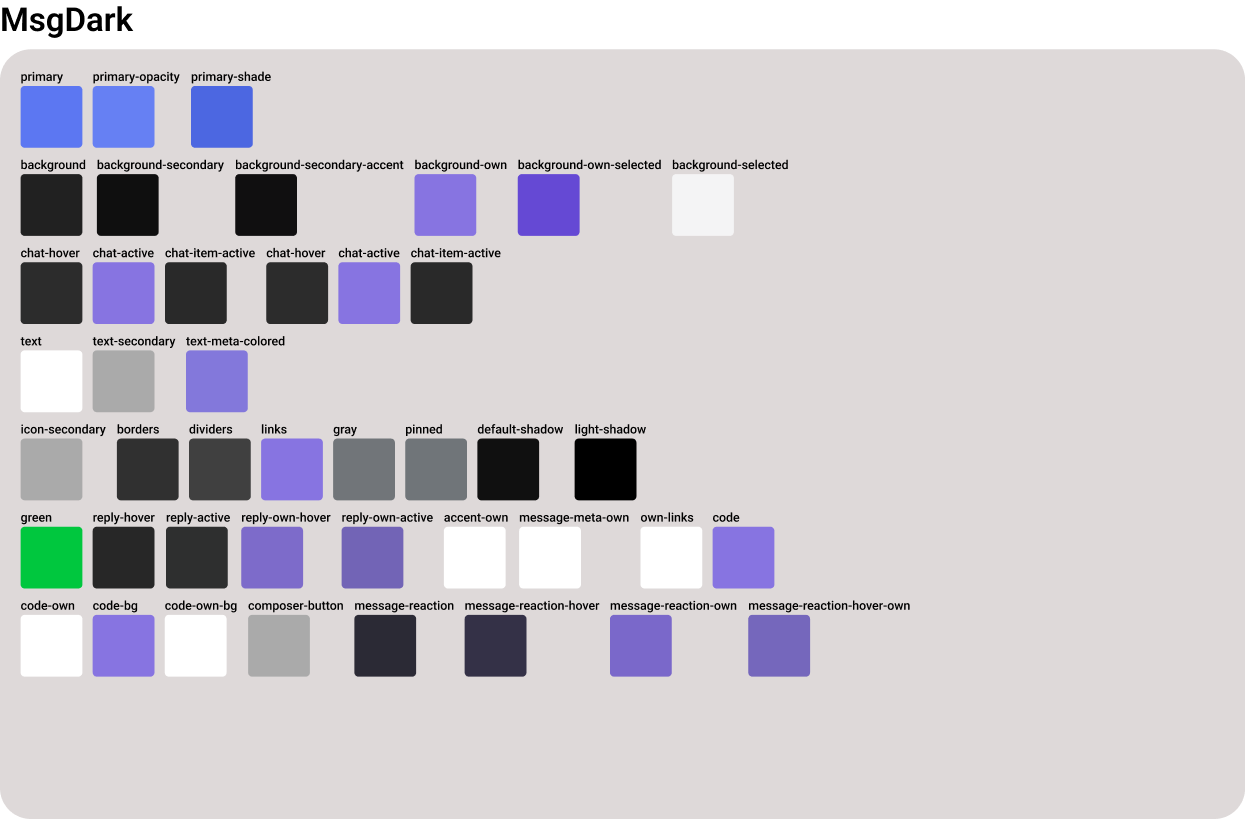
\includegraphics[width=0.75\hsize]{fig/msg-color-schema.png}\\[2mm]
\caption{Пример темной цветовой схемы}\label{fig:msg-color-schema}
\end{center}
\end{figure}

\begin{figure}[H]
\begin{center}
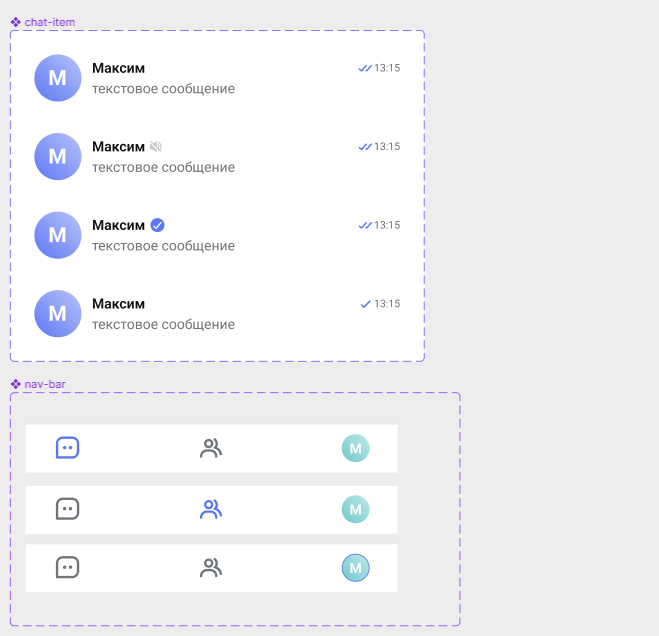
\includegraphics[width=0.7\hsize]{fig/msg-compoentns.png}\\[2mm]
\caption{Пример спроектированных компонентов}\label{fig:msg-components}
\end{center}
\end{figure}

Были спроектированы все экраны веб-приложения, экраны проектировались для мобильных и настольных устройств. Пример спроектированного экрана для мобильных и настольных устройств показан на рисунке \ref{fig:msg-adaptive}. При проектировании использовался подход «mobile first», который подразумевает в первую очередь разработку мобильной версии веб-приложения, в виду того, что адаптация мобильной версии к настольной является более простой, нежели наоборот. В виду того, что разрабатываемая коммуникационная система является корпоративной, ожидается, что количество пользователей с настольными устройствами также будет велико, поэтому дизайн одинаково пристально проектировался как для мобильных, так и для настольных устройств. Примеры различных спроектированных экранов веб-приложения показаны на рисунках \ref{fig:msg-auth}, \ref{fig:msg-invite}, \ref{fig:msg-common}.

\begin{figure}[H]
\begin{center}
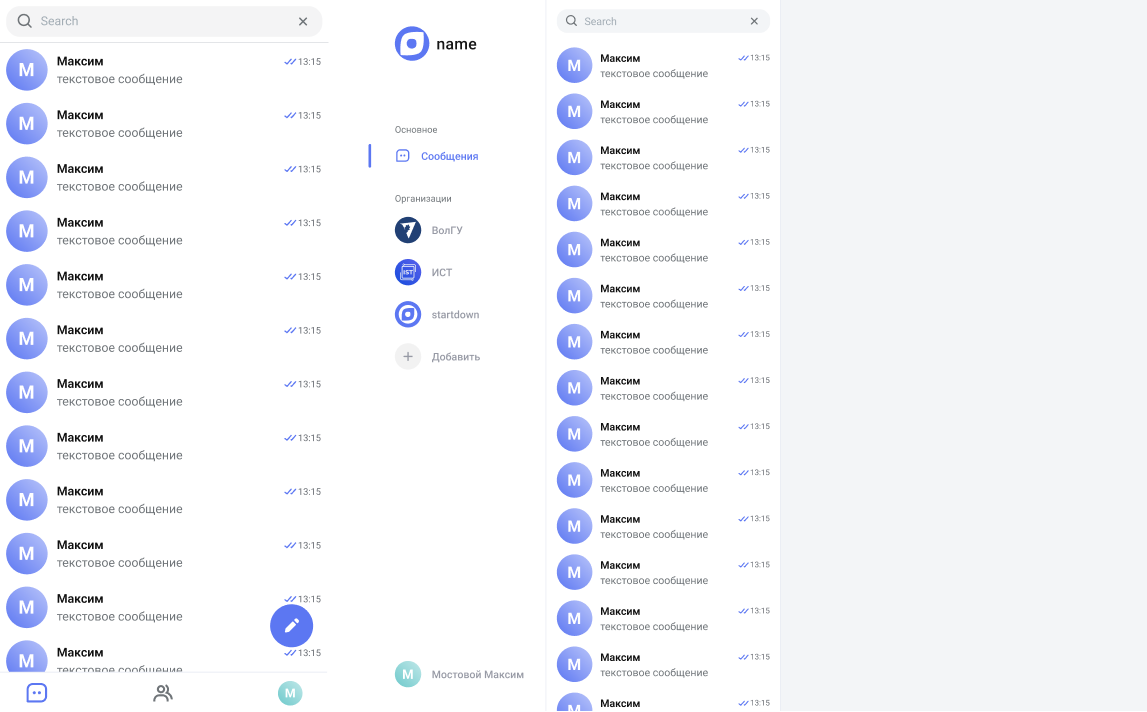
\includegraphics[width=0.8\hsize]{fig/msg-adaptive.png}\\[2mm]
\caption{Пример спроектированного экрана для мобильных и настольных устройств}\label{fig:msg-adaptive}
\end{center}
\end{figure}

\begin{figure}[H]
\begin{center}
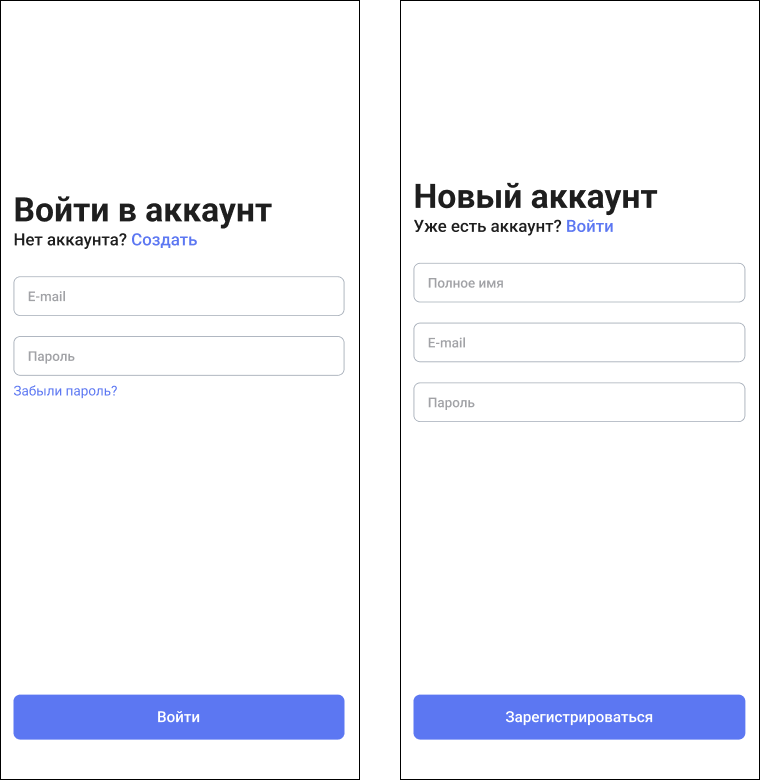
\includegraphics[width=0.5\hsize]{fig/msg-auth.png}\\[2mm]
\caption{Пример спроектированных экранов входа и регистрации}\label{fig:msg-auth}
\end{center}
\end{figure}

\begin{figure}[H]
\begin{center}
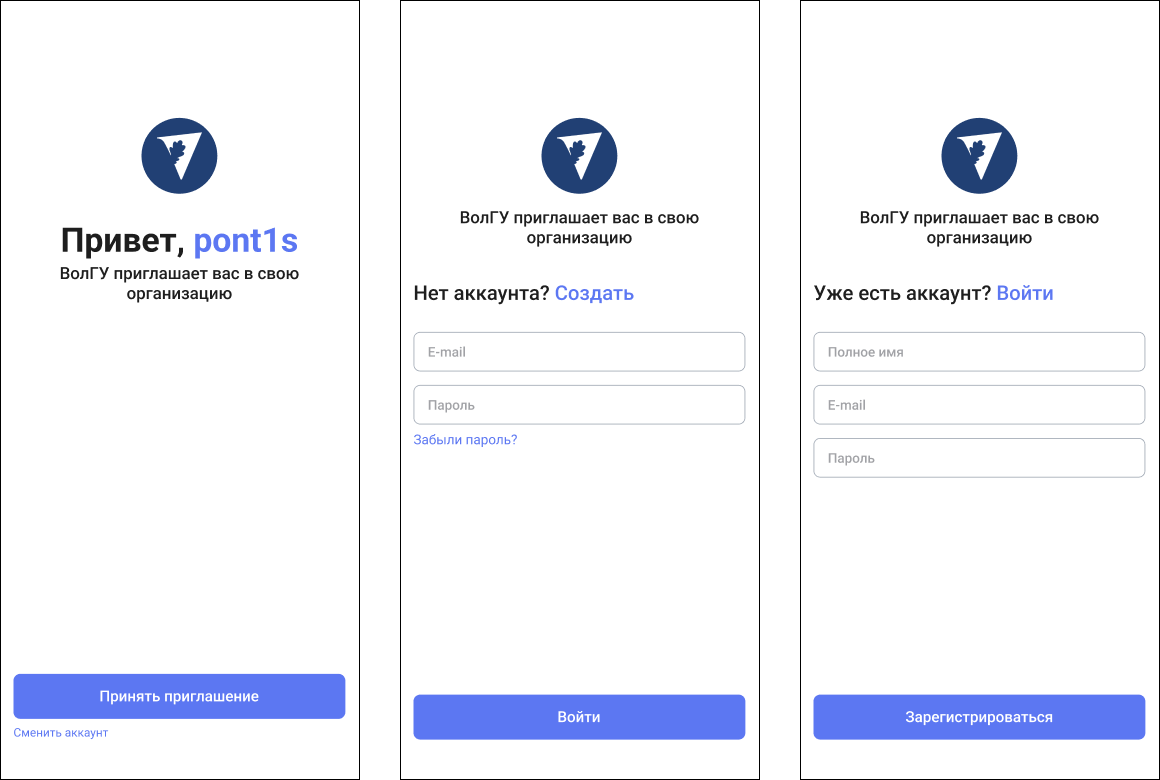
\includegraphics[width=0.8\hsize]{fig/msg-invite.png}\\[2mm]
\caption{Пример спроектированных экранов приглашения в организацию}\label{fig:msg-invite}
\end{center}
\end{figure}

\begin{figure}[H]
\begin{center}
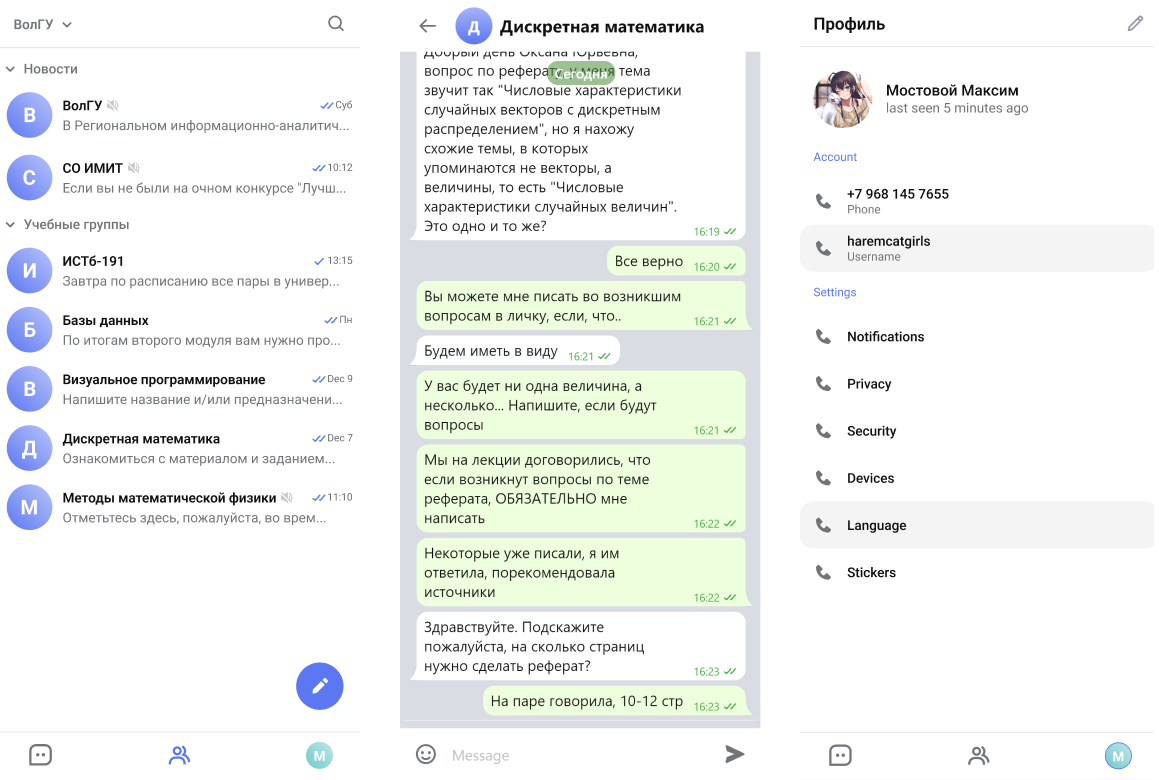
\includegraphics[width=0.8\hsize]{fig/msg-common.png}\\[2mm]
\caption{Пример спроектированных экранов организации, чата, профиля}\label{fig:msg-common}
\end{center}
\end{figure}